\section{Plugin Catalog}
\label{sec:chapter_3_section_4}

\noindent
 Il plugin catalog \`e l'elemento centrale che fornisce allo users un sistema con un ricco catalogo di plugins,
 in cui per ogni elemento presente al suo interno \`e descritto da un nome, una descrizione ed una
 immagine di anteprima del modello 3D (come si vede in Figura~\ref{fig:figura1} (a)). Quando l'utente \`e all'interno
 sceglie il plugin da inserire con un click, dopo il quale si passa nella modalit\`a 2D-view, dove verr\'a posizionato
 all'interno della scena (come si vede in Figura~\ref{fig:figura1} (b)).

% It is pivotal to provide the system users with a rich catalog of plugins, to cover all the basic as well as the most advanced modeling requirements.
% Table~\ref{tab:plugins-example} (see Figure~\ref{fig:catalog}) reports examples of plugins arranged according to the  taxonomy introduced in Section~\ref{ssec:taxonomy}.

\begin{figure}[htbp]
\begin{center}
\begin{tabular}{c @{\hspace{1em}} c}
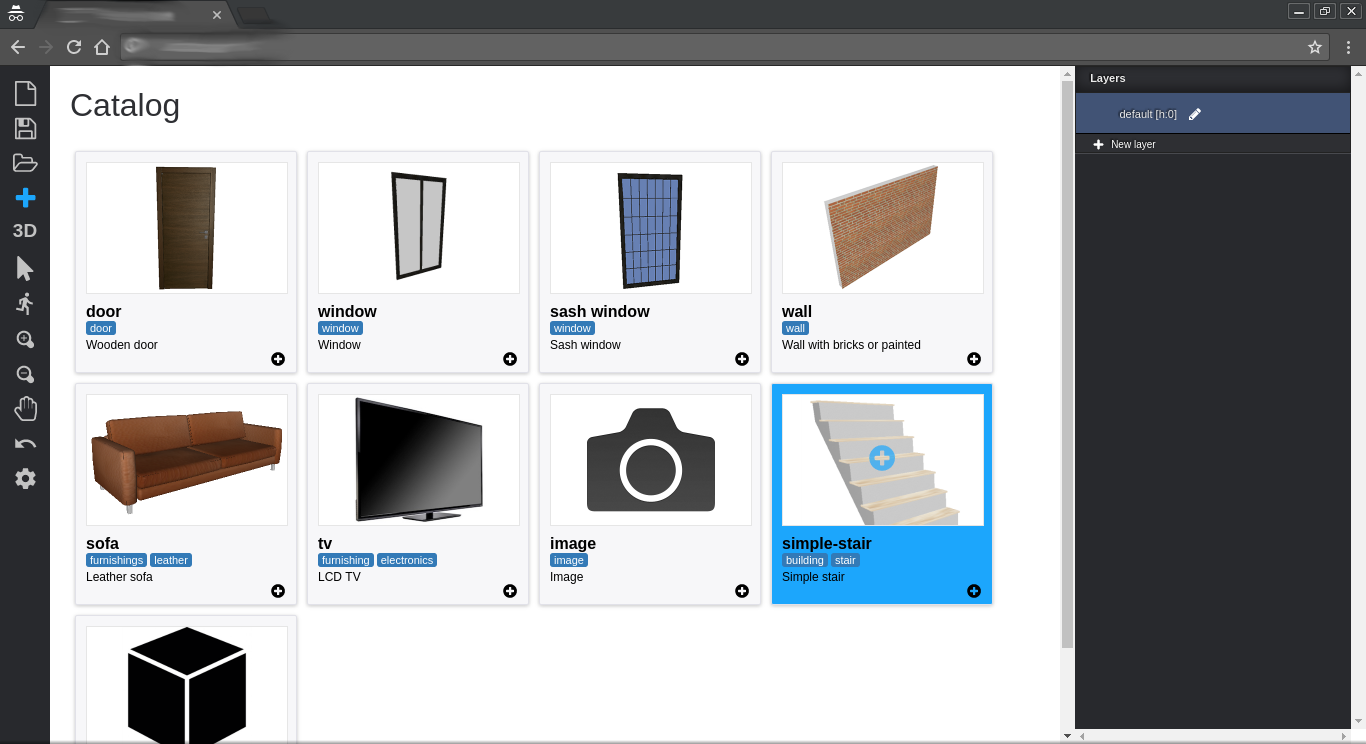
\includegraphics[width=9cm]{images/figcatalog} \\
  (a)  \\
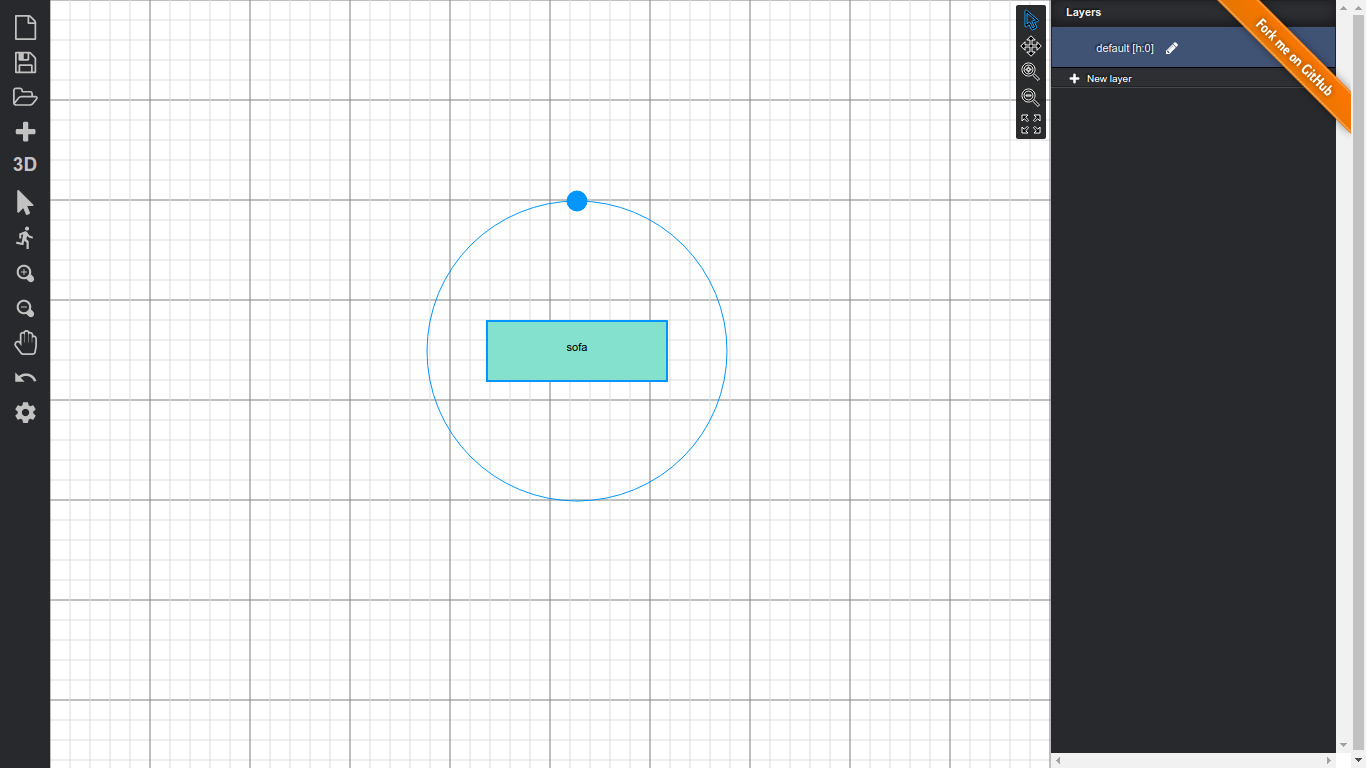
\includegraphics[width=9cm]{images/positioning} \\
  (b) \\
\end{tabular}
\end{center}
\caption{Dettaglio Plugins: (a) Vista dei plugins nel catalogo, (b) inserimento oggetto dopo la selezione nel catalogo}\label{fig:figura1}
\end{figure}
\newpage
